\if0
本章では ArchHDL での論理シミュレーションの実行時間を評価し,Icarus Verilog, NC-Verilog, VCS での論理シミュレーションの実行時間と比較する.
\fi
In this chapter, I evaluate the elapsed time of logic simulation in ArchHDL and it is compared with that of logic simulation in Icarus Verilog, NC-Verilog and VCS.

\begin{table}[t]
\if0
 \caption{実行環境}
\fi
 \caption{Simulation environment}
 \label{table:exec_env}
 \begin{center}
  \begin{tabular}{l|c|c} \hline
         &  Icarus Verilog, ArchHDL  &  NC-Verilog, VCS   \\ \hline
  OS     &  Ubuntu12.04             &  CentOS5.9        \\
  CPU    &  Core i7-3770K 3.50GHz   &  Core i7-3770K 3.50GHz  \\
\if0
  メモリ  &  $16\,\mathrm{GB}$       &  $16\,\mathrm{GB}$  \\ \hline
\fi
   Memory &  $16\,\mathrm{GB}$       &  $16\,\mathrm{GB}$  \\ \hline
  \end{tabular}
 \end{center}
\end{table}

\if0
\tabref{table:exec_env} に実行環境をまとめる.
評価には同じ仕様の 2 台の計算機を用いる.
一台は Icarus Verilog, ArchHDL の評価に用いる.もう一台は NC-Verilog, VCS の評価に用いる.
CPU,メモリなどのハードウェアの仕様は同一であるがソフトウェアの制約により異なる OS を利用する.
\fi
\tabref{table:exec_env} shows the simulation environment.
I use the two computers of the same specification for the evaluation.
I use to evaluate Icarus Verilog and ArchHDL
One computer is used to evaluate Icarus Verilog and ArchHDL.
The other is used to evaluate NC-Verilog and VCS.
The two computers are the same specification such as hardware, CPU, memory and so on.
However, I use different operating systems due to the limitations of the software.

\if0
異なる OS を用いる理由を述べる.
NC-Verilog と VCS は RedHat 系のディストリビューションのみをサポートしている.
今回は RedHat 系のディストリビューションである CentOS5.9 を用いる.
しかし CentOS5.9 に含まれる gcc のバージョンは 4.1.2 である.
\ref{s:lambda}節で述べたように,ArchHDL では C++11 のラムダ関数を用いて記述するため gcc のバージョンは 4.5 以上が必要である.
その条件を満たす Ubuntu12.04 を評価に用いる.
Ubuntu12.04 に含まれる gcc のバージョンは 4.6.3 である.
gcc の最適化オプションとして \verb/-O2/ を用いる.
Icarus Verilog はどちらのディストリビューションでも動作するが,今回は Ubuntu12.04 を用いる.
Ubuntu12.04 に含まれる Icarus Verilog のバージョンは 0.9.5 である.
VCS のバージョンは vcsC-2009.06 を用いる.NC-Verilog のバージョンは 06.20-s004 を用いる.
\fi
I describe the reason for using different operating systems.
NC-Verilog and VCS support only RPM-based Linux distributions.
I use CentOS5.9 which is RPM-based Linux distributions for this evaluation.
However, the version of GCC includes CentOS5.9 is 4.1.2.
I describe it in Section \ref{s:lambda} that the version of GCC is required 4.5 or later  for using the lambda function in ArchHDL.
I also use to evaluate the Ubuntu12.04 satisfying the condition.
The version of GCC includes Ubuntu12.04 is 4.6.3.
I use \verb/-O2/ as optimization option of GCC.
Icarus Verilog runs on both computers.
I use it on Ubuntu12.04 in this evaluation.
The version of Icarus Verilog includes Ubuntu12.04 is 0.9.5.
The version of NC-Verilog is 06.20-s004.
The version of VCS is vcsC-2009.06.

\if0
今回用いる計算機の CPU の物理コアは 4 コアであるため, OpenMP による並列化はスレッド数を 8 個にして評価する.
\fi
Because physical cores of the CPU of the computers are 4 cores for this evaluation,
I evaluate the parallelization with OpenMP in 8 threads

\if0
評価では,2 つのマイクロベンチマークと,現実的なハードウェアのベンチマークとしてステンシル計算回路\cite{koba:stencil}を用いる.
Verilog HDL と ArchHDL のためのハードウェアシミュレーションは手作業により作成した.
両ハードウェアシミュレーションの出力は同様になるように作成した.
\fi
In the evaluation, I use two micro benchmarks
and stencil-computation circuit as a benchmark of hardware realistic.
I have created hardware simulation for ArchHDL and Verilog HDL by myself
and the output of both the hardware simulation to be same.

\if0
評価結果に用いているラベルの名前について述べる.
オリジナルの ArchHDL は \textbf{ArchHDL} と表す.
\ref{sss:no_set} 節で述べた条件分岐の除去を適用したものを \textbf{NO SET} と表す.
\ref{sss:mem_copy} 節で述べたメモリ配置の工夫を適用したものを \textbf{MEM MAP} と表す.
\ref{ss:parallel} 節で述べた並列化を行ったものを \textbf{PARA} と表す.
メモリ配置の工夫と並列を同時に適用したものを \textbf{MEM MAP + PARA} と表す.
\fi
I describe the name of the labels which are used on the evaluation results.
Original ArchHDL is named \textbf{ArchHDL}.
It is named \textbf{NO SET} that I apply removal of the conditional branch to ArchHDL, which is described in Section \ref{sss:no_set}.
It is named \textbf{MEM MAP} that I apply devising a memory allocation and stored as an array to ArchHDL, which is described in Section \ref{sss:mem_copy}
It is named \textbf{PARA} that I apply the parallelization to ArchHDL, which is described in Section \ref{ss:parallel}.


\section{Evaluation by Micro Benchmark}

マイクロベンチマークとしてカウンタ回路と XORSHIFT による乱数生成回路を用いる.

\begin{figure}[tb]
 \lstinputlisting[language=c++]{src/xorshift_alg.cc}
\if0
 \caption{XORSHIFT 法に基づく乱数生成のアルゴリズム}
\fi
 \caption{Algorithm of random number generation based on xorshift RNG}
 \label{src:xorshift_alg}
\end{figure}

カウンタ回路とは \figref{src:counter} に示した 1 サイクルごとに 1 を足す回路である.
ハードウェアの規模を増やすためにカウンタの数を指定できるようにした.
XORSHIFT による乱数生成回路とはシフトと XOR 演算のみで構成できる XORSHIFT 法に基づく乱数生成器をハードウェア記述によって実装した回路である.
\figref{src:xorshift_alg} に XORSHIFT 法に基づく乱数生成のアルゴリズムを C 言語によって実装したものを示す.

\begin{figure}[tb]
 \centering
 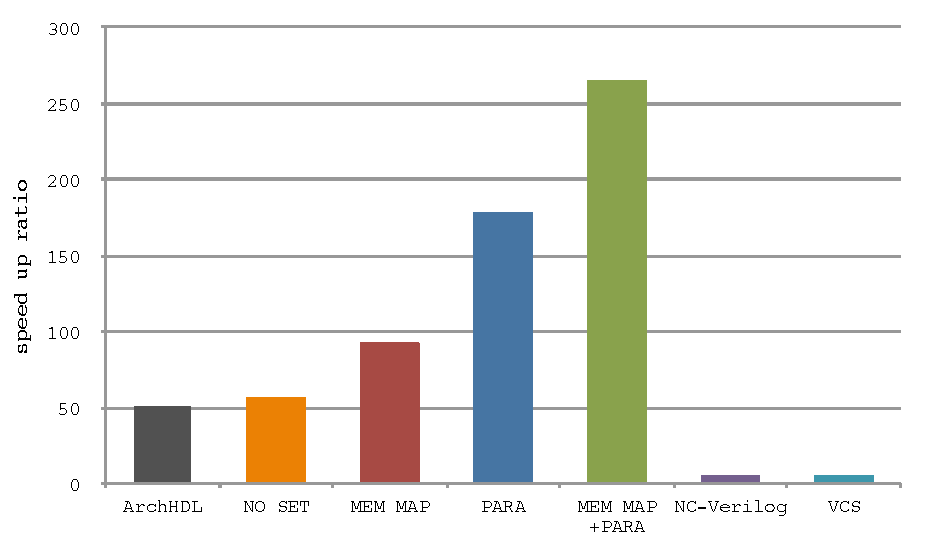
\includegraphics[clip,width=\linewidth]{counter_4096}
\if0
 \caption{4096 個のカウンタ回路の実行時間を Icarus Verilog と比較した速度向上比}
\fi
 \caption{Speed up ratio compared with the elapsed time of 4096 of the counter circuit with Icarus Verilog}
 \label{fig:counter4096}
\end{figure}

\figref{fig:counter4096} に 4096 個のカウンタ回路の実行時間を Icarus Verilog と比較した速度向上比を示す.
縦軸は Icarus Verilog での実行時間を 1 とした速度向上比を示している.

ArchHDL は商用の NC-Verilog, VCS と比較してもかなり高速である.
\textbf{MEM MAP + PARA} の論理シミュレーション実行時間は NC-Verilog の 58.8 倍,VCS の 56.7 倍高速である.

また今回提案している高速化手法はオリジナルの ArchHDL に比べていずれも効果が出ている.
\textbf{MEM MAP + PARA} の論理シミュレーション実行時間はオリジナルの ArchHDL の 5.23 倍高速である.



\begin{figure}[tb]
 \centering
 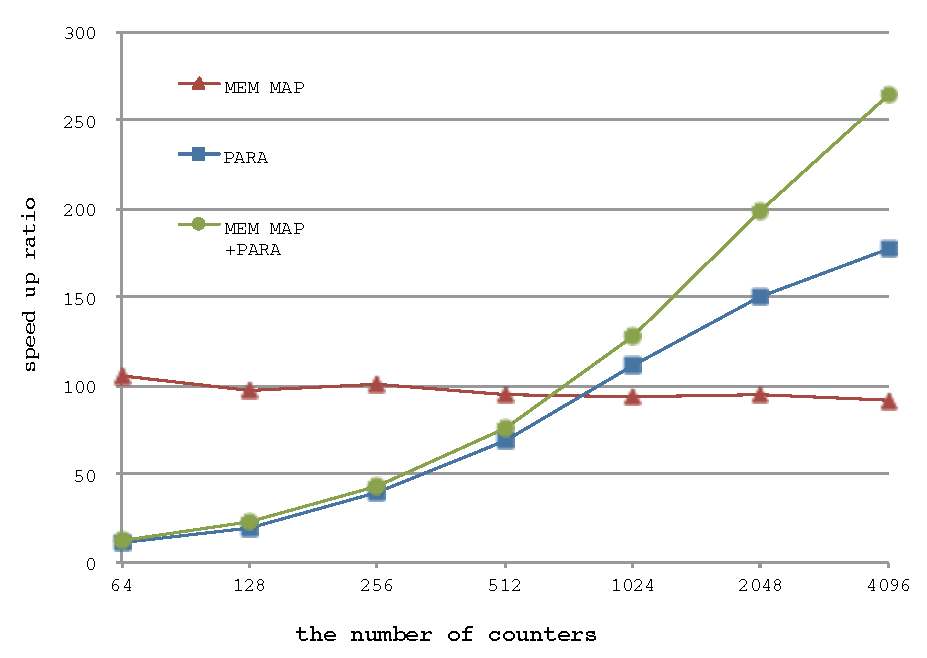
\includegraphics[clip,width=\linewidth]{counter_con}
\if0
 \caption{高速化手法を適用した ArchHDL と OpenMP を適用したカウンタ回路の実行時間を Icarus Verilog と比較した速度向上比}
\fi
 \caption{Speed up ratio compared with the elapsed time of the counter circuits with Icarus Verilog in ArchHDL applying the fast method and OpenMP}
 \label{fig:counter_con}
\end{figure}

\figref{fig:counter_con} に高速化手法を適用した ArchHDL と OpenMP を適用したカウンタ回路の実行時間を Icarus Verilog と比較した速度向上比を示す.
縦軸は Icarus Verilog での実行時間を 1 とした速度向上比を示している.
横軸はカウンタの個数である.

\textbf{MEM MAP} は逐次に実行されているので Icarus Verilog と比較した速度向上比はカウンタの個数を変えてもほとんど変わらない.
並列化を行った \textbf{PARA} と \textbf{MEM MAP + PARA} はカウンタの個数が 1024 個以上で \textbf{MEM MAP} よりも高速になる.
\textbf{PARA} より \textbf{MEM MAP + PARA} の方が常に高速であるので今回提案している逐次処理での高速化手法は並列化を行った場合でも効果が出ている.
カウンタの個数はハードウェアの規模とみなせるため,並列化が有効なのはある程度規模の大きい回路であると言える.


\begin{figure}[tb]
 \centering
 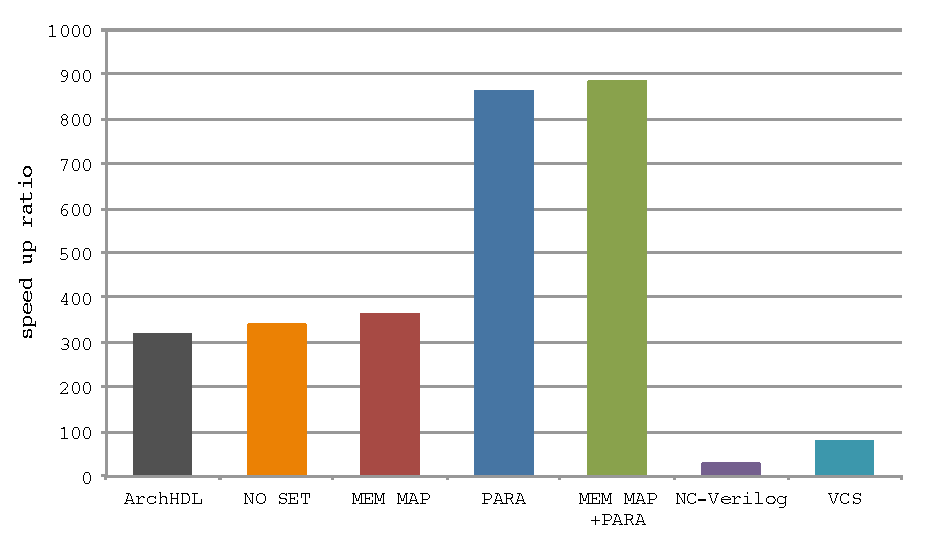
\includegraphics[clip,width=\linewidth]{xorshift}
\if0
 \caption{512 個の XORSHIFT による乱数生成器の実行時間を Icarus Verilog と比較した速度向上比}
\fi
 \caption{Speed up ratio compared with the elapsed time of 512 of the random number generator circuits by XORSHIFT RNG with Icarus Verilog}
 \label{fig:xorshift}
\end{figure}

\figref{fig:xorshift} は XORSHIFT による乱数生成器での実行時間を Icarus Verilog と比較した速度向上比である.
試行回数は 524,288 回である.初期値の異なる乱数生成器を 512 個用意している.

ArchHDL は商用の NC-Verilog, VCS と比較してもかなり高速である.
\textbf{MEM MAP + PARA} の論理シミュレーション実行時間は NC-Verilog の 32.2 倍,VCS の 11.3 倍高速である.

また今回提案している高速化手法はオリジナルの ArchHDL に比べていずれも効果が出ている.
\textbf{MEM MAP + PARA} の論理シミュレーション実行時間はオリジナルの ArchHDL の 2.78 倍高速である.


\section{Evaluation by Stencil-Computation Circuit}

\if0

\begin{table}[tb]
 \caption{ステンシル計算回路でのプロファイリング結果 1.1}
 \label{table:stencil_prof1.1}
 \begin{center}
  % \setlength{\tabcolsep}{3pt}
  \begin{tabular}{lr} \toprule
  関数名 & 実行時間に占める割合 (\%) \\ \midrule
  reg::Update() (合計) & 16.57 \\
  ArchHDL::Step() & 12.47 \\
  brk & 15.05 \\ \bottomrule
  \end{tabular}
 \end{center}
\end{table}

\fi

\begin{figure}[tb]
 \centering
 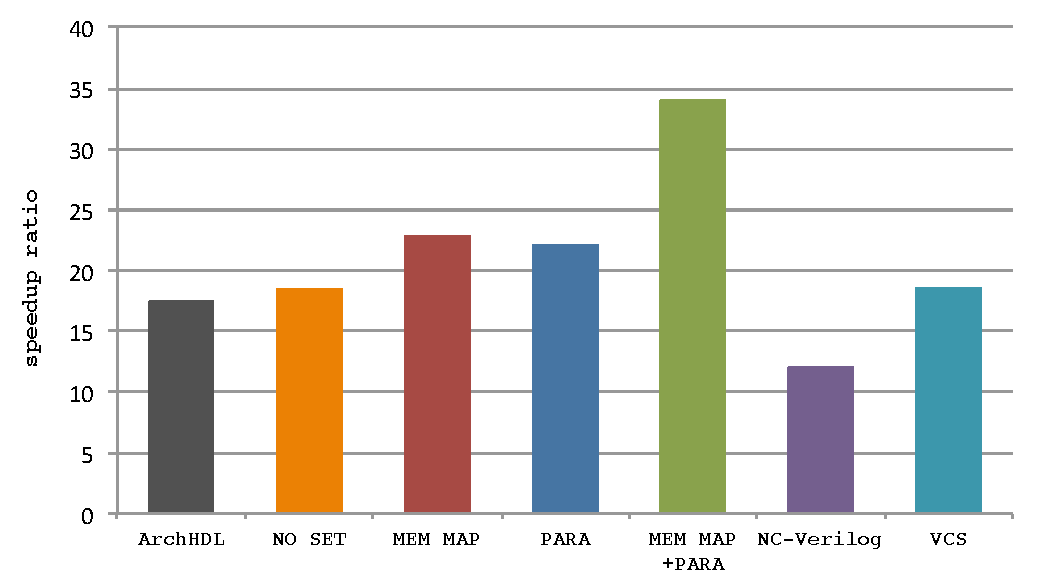
\includegraphics[clip,width=\linewidth]{stencil}
\if0
 \caption{ステンシル計算回路の Icarus Verilog と比較した実行時間の速度向上比}
\fi
 \caption{Speed up ratio compared with the elapsed time of a stencil-computation circuit with Icarus Verilog}
 \label{fig:stencil}
\end{figure}

\figref{fig:stencil} はステンシル計算回路での実行結果である.
縦軸は Icarus Verilog と比較したそれぞれの速度向上比である.

オリジナルの ArchHDL は商用の NC-Verilog より高速であったが,同じく商用の VCS はオリジナルの ArchHDL と \textbf{NO SET} より高速である.
しかし逐次実行での高速化手法と並列化を共に適用した \textbf{MEM MAP + PARA} の論理シミュレーション実行時間は VCS の 1.83 倍高速である.

ステンシル計算回路の場合は Update() は 325,469,175 回呼ばれているのに対して,
reg の値に更新がないのは 5,145,760 回である.
つまり更新がないのは Update() メソッド呼び出し全体の $1.58\%$ 程度に過ぎない.
それにより条件分岐を無くす \textbf{NO SET} の論理シミュレーションはオリジナルの ArchHDL より高速である.
また Update() のメソッド呼び出しを減らし,かつメモリ配置を工夫している \textbf{MEM MAP} の論理シミュレーション実行時間はオリジナルの ArchHDL の 1.31 倍高速である.

また Module が 133 個,reg が 991 個存在する回路なので並列化の効果も大きい.
逐次実行での高速化手法と並列化を共に適用した \textbf{MEM MAP + PARA} の論理シミュレーション実行時間はオリジナルの ArchHDL の 1.95 倍高速である.


% \subsection{高速化の解析}
